%!TEX ROOT = thesis.tex
\chapter{Introduction}
\section{Basic Introduction}
Exchange rates can be defined as the values which are used for  converting one currency to another currency. Exchange rates are influenced by many factors such as economic situations and political changes, and also the psychological states of individual  who involved in trading and investing in the financial markets. Forecasting exchange rates is useful for governments, companies, and individuals in making decisions on their investments and trading. It can help the traders with their decisions to behave in the markets. Companies also have competitive advantages by having  the ability to predict  future exchange rates for  making  successful market decisions.

Forecasting the exchange rates is not a simple task due to its complex correlations with the factors that influenced by. Their interactions are complex, dynamic and  unstable  manners.There are many approaches exist for forecasting exchange rates. There are many types of forecasting methods which applied technical analysis approach  such as causal forecasting,time series forecasting and so on. This project mainly focuses on technical  analysis approach. Technical analysis approach performs the prediction by analyzing the past behaviors of the data and, identifying the patterns within it, and makes the predictions on the  behaviors  in the future. 

 Forecasting in financial markets, in general, can be considered as time series forecasting since it is based on historical datasets.The main advantage of time series prediction is that it can explain  the past and predict the future behaviors of particular interest  of variable. There are two methods of time series forecasting. The two methods of time series forecasting are linear and nonlinear. The  mostly used methods, as well as conventional  statistical methods  in linear time series forecasting, are regression methods, and  ARIMA (Autoregressive Integrated Moving Average) methods. ARIMA is also called Box-Jenkins methods. ARIMA is used to fit data to the time series to get a better understanding of the data or to predict the future points of the data in the time series.

However, it does not fit to use linear methods for forecasting of exchange rates due to its complex, dynamic natures. Hence, this project focuses on the  nonlinear time series forecasting methods. Nonlinear times series methods are applied in most of the  forecasting which complex and dynamic nature of behaviors exist. When it comes to nonlinearity, one the most popular which are being applied in current application is Artificial Neural Networks (ANNs) methods.

ANNs is  a system of interconnected neurons  or nodes. The Inspiration of ANNs comes from the biological human brain.The human brain has billions of interconnected neurons which have the ability to learn and grow over time. A single neuron is equivalent to a single processing unit  in computer term. The idea of ANNs is  to mimic the features which have  in biological neurons to give  machines the ability to learn. A biological neuron has the combination of an axon, synapse, and dendrite. According to \citeA{beale:1990}, the basic features of a biological neuron is shown in the figure 1.1.

\begin{figure}[hbt!]\centering
	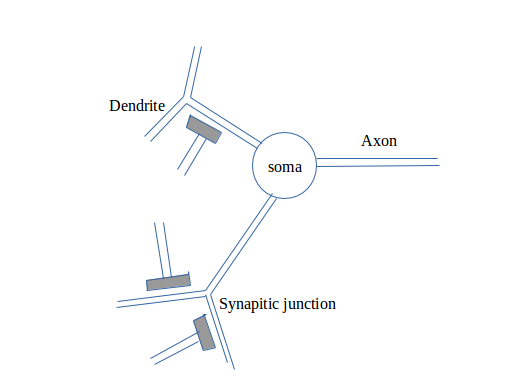
\includegraphics[width=.6\textwidth]{basic_neuron}
	\caption{The basic features of a biological neuron}
\end{figure}

In a biological neuron, the dendrites  serve as the input vector. Each dendrite is able to do multiplication by that dendrite's weight value. The soma does as the summation function  and produces a signal. As the signals arrive in the soma from the dendrites, the positive and negative signals are effectively added in the summation function or the soma. The axon gets its signal from the summation results which happens inside the soma. When the soma reaches a certain value, the axon will transmit a signal pulse down its length.

According to \citeA{haykin:1994}, the three basic elements of the artificial neuron model are : 
\begin{enumerate}
	\item A set of  inputs which is attached to weights.
	\item A summation  for the input signals weighted
	\item An activation or transfer function which used to  limit  the output.
\end{enumerate}


The mathematical representation can be shown as below. 

\begin{equation*}
	X = f_h[\sum_{i=0}^n (w_ix_i)]
\end{equation*}
\\
where\\
X = the output of the neuron \\ 
$f_h$ = the activation function \\
$w_i$ = the weights \\
$x_i$ = the inputs

The graphical representation of the single neuron is illustrated in the figure 1.2.
\begin{figure}[hbt!]\centering
	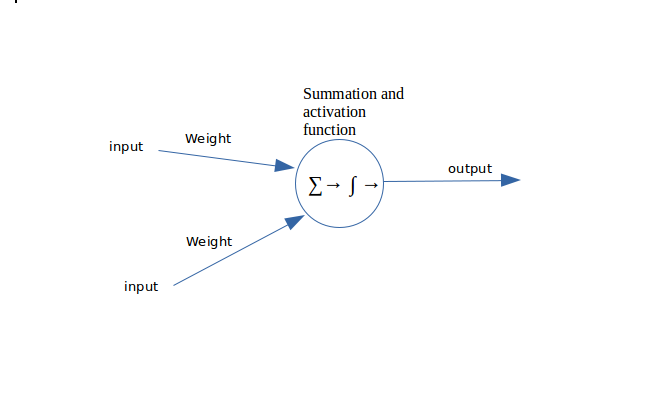
\includegraphics[width=.6\textwidth]{basic_model}
	\caption{Basic artificial neuron  model }
\end{figure}

ANNs have different ways of construction of a network. ANNs have a capability that makes them significantly different compared to standard computing. ANNs belong to the class of data-driven approaches \cite{talati:2000}. In data driven approaches, data is of importance  to achieve a neural network which fits the data well. The main advantage of ANNs is the ability to learn and generalize from the training dataset to predict future values.  

The most applied ANNs methods in forecasting exchange rates are feed-forward  neural network and recurrent neural network which are in  supervised learning paradigm. In the supervised learning paradigm, the right answers are given to the network, so that it can calculate the errors between desired outputs and actual outputs. This project focuses on the supervised learning paradigm. 

\section{Problem Statement }
The forecasting of foreign exchange rates plays a main role in the international  business and banking decision making, especially in today's global business environment. It is proposed to predict the future exchange rates by extracting regularities from observations of past exchange rates. Artificial Neural Networks (ANNs) has been extensively used for forecasting applications. This project focuses mainly on the  optimal ANN models and ensemble  the different models to get better performance than a  single optimal model.

The optimal ANNs model is normally selected based on the architecture which produces better performance on the testing data set. The model selected may not be the true optimal model in the sense that infinite variations that can be provided for different parameters cannot be tested completely in determining the optimal model. In this project, it is proposed to combine the outputs of several individual neural network models or construct the multi-stage ensemble neural network model for forecasting and then compare the performance with the single NN model.

\section{Scope}
The project is mainly focused on supervised learning paradigm which widely used for exchange rates forecasting application. There is another type learning paradigm which is not in the scope of this project is unsupervised learning. The project will be based on the most popular methods for forecasting using ANNs which are  Multilayer Perceptrons(MLPs), Recurrent Neural Network (RNN), and Radial Basic Functions (RBF). Researchers have shown these methods have reasonable performance compared to other forecasting methods. These three methods will be ensembling  with different types of learning functions, as well as activation or transfer functions.
\section{Project objectives }
The objectives of this project are: 
\begin{enumerate}
	\item To predict  future values of exchange rates by using its time series dataset.
	\item To  construct  ensemble artificial  neural network model by constructing  MLPs, RNN, and RBF neural network with different learning algorithms and activation functions.
	\item To compare the performance of the ensemble homogeneous artificial neural network and heterogeneous ANN model with single optimal ANN models.
\end{enumerate}

